\section{Diseño Detallado}

\subsection{Comunicación Humano Máquina (Sistema de Alimentación)}

El módulo de comunicación Humano-Máquina se propone realizar a través de una interfaz gráfica como lo es el \textit{display} Nextion, su selección es debido a su resolución y tamaño, junto a que es una pantalla táctil, reduciendo la cantidad de periféricos necesarios para lograr ingresar datos al sistema. 

En la tabla \ref{tab:MMHMI} se muestra más a detalle la comparación de las opciones disponibles.

\begin{table}[htbp]
\centering
\caption{Matriz morfológica de selección de display}
\label{tab:MMHMI}
\resizebox{\textwidth}{!}{%
\begin{tabular}{|l|l|l|l|l|l|l|l|}
\hline
Criterio         & Peso   & LCD      & P    & OLED     & P   & NEXTION & P   \\ \hline
Tamaño           & $25\%$ & 3.2''    & 4    & 2.4''    & 3   & 3.5''   & 5   \\ \hline
Consumo          & $20\%$ & \SI{5}{\volt}      & 2    & \SI{4.06}{\volt}    & 4   & \SI{5.02}{\volt}    & 2   \\ \hline
Resolución                                                                 & $10\%$ & $128\times64$ px & 3 & $128\times64$ px & 3 & $480\times320$ px & 3 \\ \hline
Costo            & $15\%$ & $\$150$  & 5    & $\$253$  & 3   & $\$840$ & 1   \\ \hline
Facilidad de uso & $15\%$ & Moderada & 3    & Moderada & 3   & Fácil   & 5   \\ \hline
\begin{tabular}[c]{@{}l@{}}Uso específico \\ (Ingresar datos)\end{tabular} & $15\%$ & Difícil          & 3 & Moderada         & 1 & Fácil             & 5 \\ \hline
Totales          &        &          & 3.35 &          & 2.9 &         & 3.6 \\ \hline
\end{tabular}%
}
\end{table}


\subsection{Almacenamiento del alimento}

Para el diseño mecánico y estructural del módulo de alimentación, se decide utilizar como base un armazón o estructura similar al utilizado en el alimentador de perros encontrado en un trabajo anterior \cite{torquemada}, para el almacenamiento y el pesaje del mismo.

En la imagen \ref{fig:Tolva Fija} se muestra el dibujo de la tolva de almacenamiento \index{tolva!de almacenamiento}. Se define una capacidad de almacenamiento máximo de $30 \text{ kg}$ de alimento en la tolva principal, eligiendo utilizar láminas de acero galvanizado \index{acero galvanizado} calibre $18$, un material popular para la construcción de tolvas, debido a las ventajas que presenta. El recubrimiento de zinc lo hace un material resistente a la corrosión y la oxidación, dando una vida útil larga. No presenta un riesgo para los animales, ya que es fácil de mantener y no reacciona al contacto con los alimentos, manteniéndolos libres de contaminantes, entre otras ventajas que el material presenta.

\begin{figure}[htbp]
    \centering
    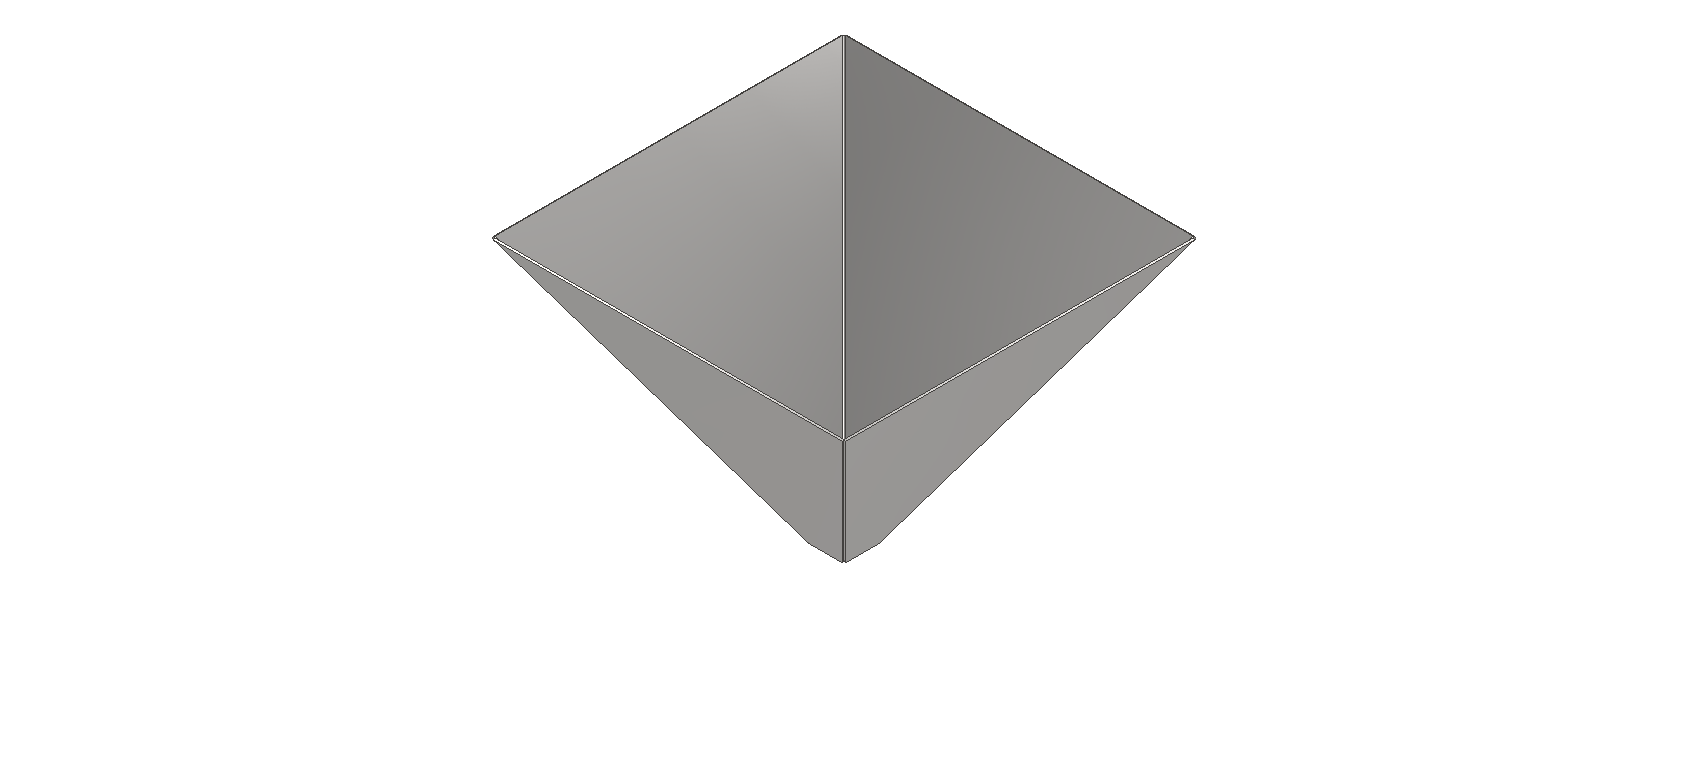
\includegraphics[width=\linewidth]{imagenes/imacap/disdet/sisalim/TolvaFija.png}
    \caption{Modelo Tolva Fija}
    \label{fig:Tolva Fija}
\end{figure}

Se realizó un experimento de medición de masa respecto a un volumen de alimento, en el que se obtuvo una densidad $\rho$ aproximada de $584 \text{ kg} / \text{m}^3$. Utilizando la definición de densidad:

$$\rho=\frac{m}{V}$$

Tenemos que el volumen necesario para contener los $30 \text{ kg}$ debe ser de $V=0.0514\text{ m}^3$. 

De acuerdo a \cite{hidalgoaznar-2022} y \cite{amoros-2001}, tenemos que en el diseño de tolvas es importante el ángulo de salida, que debe ser mayor al ángulo de reposo. Los valores típicos están entre los $50^\circ$ y $60^\circ$. Se propone un tamaño de apertura en la salida de $6 \text{ cm}$ por lado.

Partiendo de la fórmula para calcular el volumen de una pirámide truncada, se determina el valor del área superior y de la altura. Teniendo los valores de $3600 \text{ cm}^2$ y $45 \text{ cm}$ respectivamente. Verificando que el ángulo de salida se encuentra en $59^\circ$, que permite el paso del material evitando que se atore.

Para la estructura que soporta la tolva principal, imagen \ref{fig:SopTolvaFija}, se escoge el uso de PTR cuadrado de $2 \text{ pulgadas}$; ya que presenta una distribución uniforme de cargas, lo que contribuye a la estabilidad y eficiencia de la estructura; alta resistencia estructural, que garantiza la capacidad de soportar cargas significativas; y resistencia a la corrosión, asegurando durabilidad en la estructura. Así mismo, es un material que se utiliza mucho en la realización de estructuras, debido a que es fácil de soldar, cortar y perforar.

\begin{figure}[htbp]
    \centering
    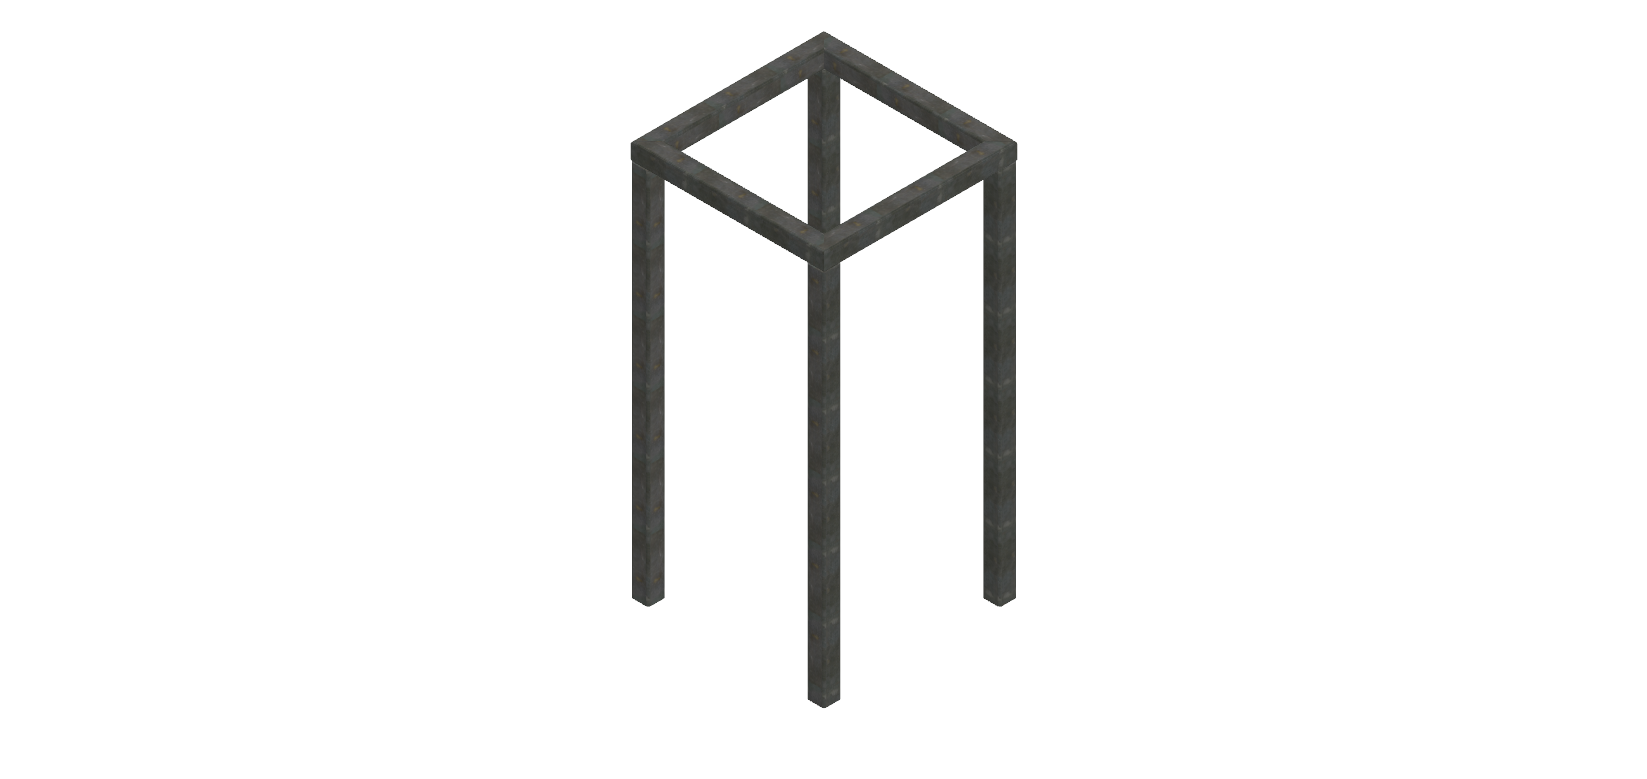
\includegraphics[width=1\linewidth]{imagenes/imacap/disdet/sisalim/EstructuraSopPrinc.png}
    \caption{Modelo de la estructura soporte de almacenamiento}
    \label{fig:SopTolvaFija}
\end{figure}

Esta estructura también soportará los componentes de los demás módulos, utilizando placas de acero de $2 \text{ mm}$ de espesor soldadas a la estructura principal.

Finalmente se calculó un motor con un par de $10.44 \text{ Nm}$ para liberar y obstruir el alimento hacia el módulo de pesaje. Este motor estará conectado con un mecanismo de piñón-cremallera que liberará y obstruirá el paso del alimento hacia el módulo de pesaje de alimento. El motor seleccionado es el NEMA 34, el cual tiene la fuerza suficiente para la apertura y cierre en la tolva fija.

\subsubsection{Validación del módulo de almacenamiento}

Se realizó un análisis de tensión utilizando el software Autodesk Inventor. Los resultados obtenidos, mostrados en la imagen \ref{fig:TVMTF}, indican que el diseño es capaz de soportar la presión ejercida por el peso del alimento sin presentar deformaciones significativas. Mostrando una tensión máxima de $680\times10^{-6} \text{ MPa}$ 

Esto demuestra que los valores de tensión se mantienen por debajo del límite elástico del material, de $207 \text{ MPa} $ garantizando la integridad estructural del diseño bajo las condiciones de carga previstas. La simulación confirma que el material y la geometría seleccionados son adecuados para contener el alimento. 


\begin{figure}[htbp]
    \centering
    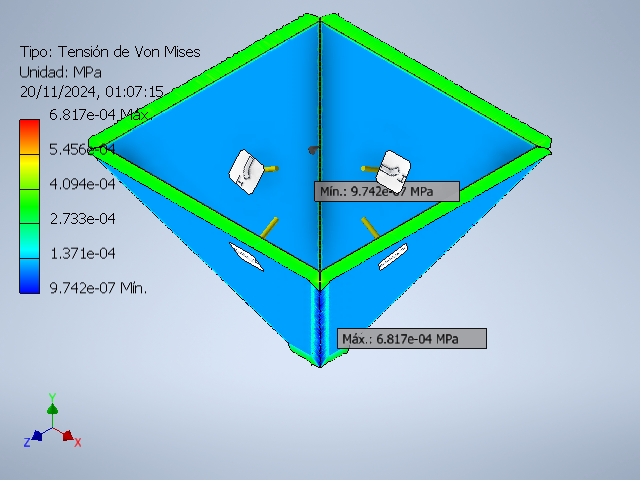
\includegraphics[width=0.8\linewidth]{imagenes/imacap/disdet/sisalim/TVMTF.png}
    \caption{Tensión de Von Mises de la tolva fija.}
    \label{fig:TVMTF}
\end{figure}

En la imagen \ref{fig:TVMSP} se muestra la simulación del análisis de elementos finitos de tensión, comprobando su resistencia al peso del alimento y la tolva, con valores muy por debajo del límite elástico del material,  $207 \text{ MPa} $, validando así la resistencia estructural mencionada. Con esta validación se asegura que la estructura es adecuada y también que se tiene un margen de seguridad considerable. 

\begin{figure}[htbp]
    \centering
    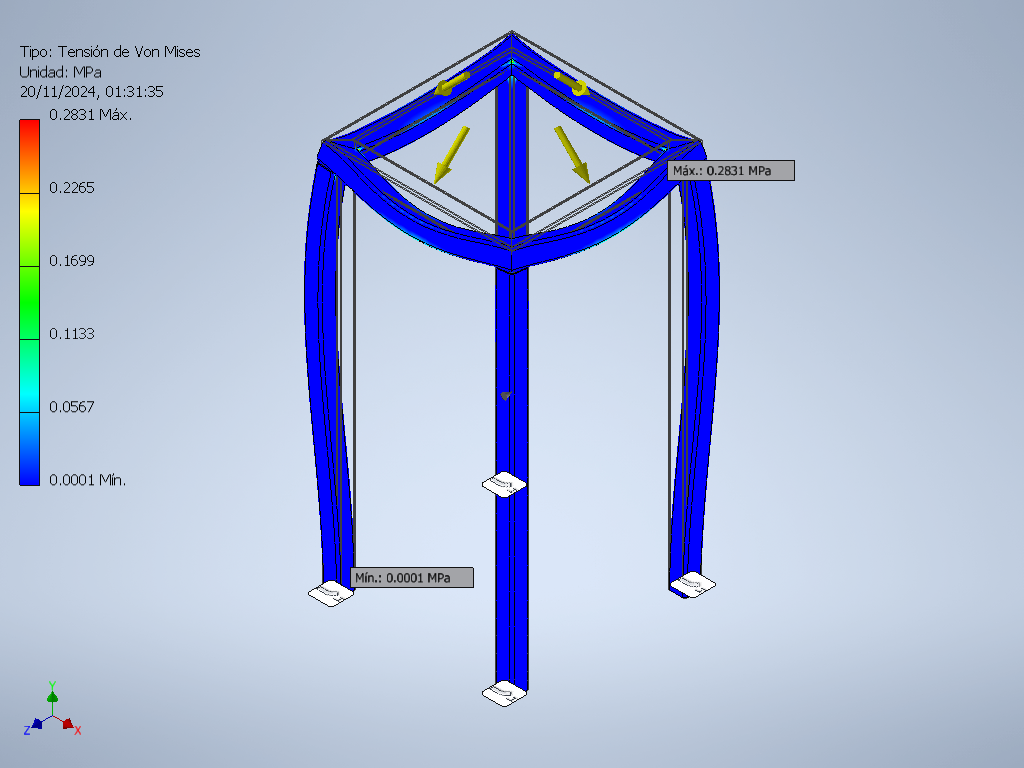
\includegraphics[width=0.8\linewidth]{imagenes/imacap/disdet/sisalim/TVMSP.png}
    \caption{Tensión de Von Mises de la estructura principal.}
    \label{fig:TVMSP}
\end{figure}

\subsection{Pesaje alimento}

Se decide realizar un sistema de pesaje del alimento o báscula \index{báscula}, para medir la cantidad de alimento que será distribuido, como se muestra en la imagen \ref{fig:Basc}. Este sistema consta de los siguientes componentes:

\begin{itemize}
    \item \textbf{Báscula:} Formada por un sensor de peso, celda de carga, y una lámina, encargados de medir el peso del alimento.
    \item \textbf{Paredes:} La báscula está rodeada por tres paredes de lámina de acero galvanizado, que actúan como barreras para mantener el alimento en su lugar durante el pesaje y como soporte del espárrago que moverá la pared móvil.
    \item \textbf{Pared Móvil:} Una pared móvil se encarga de empujar el alimento pesado hacia una rampa. Esta pared es accionada por un espárrago, que proporciona un movimiento controlado.
\end{itemize}

Este diseño garantiza un pesaje del alimento y un manejo del mismo, integrando una solución para el proceso general; en la imagen \ref{fig:Basc} se muestra la integración de los elementos del módulo.

\begin{figure}[htbp]
    \subfigure[Vista isométrica del módulo de pesaje.]{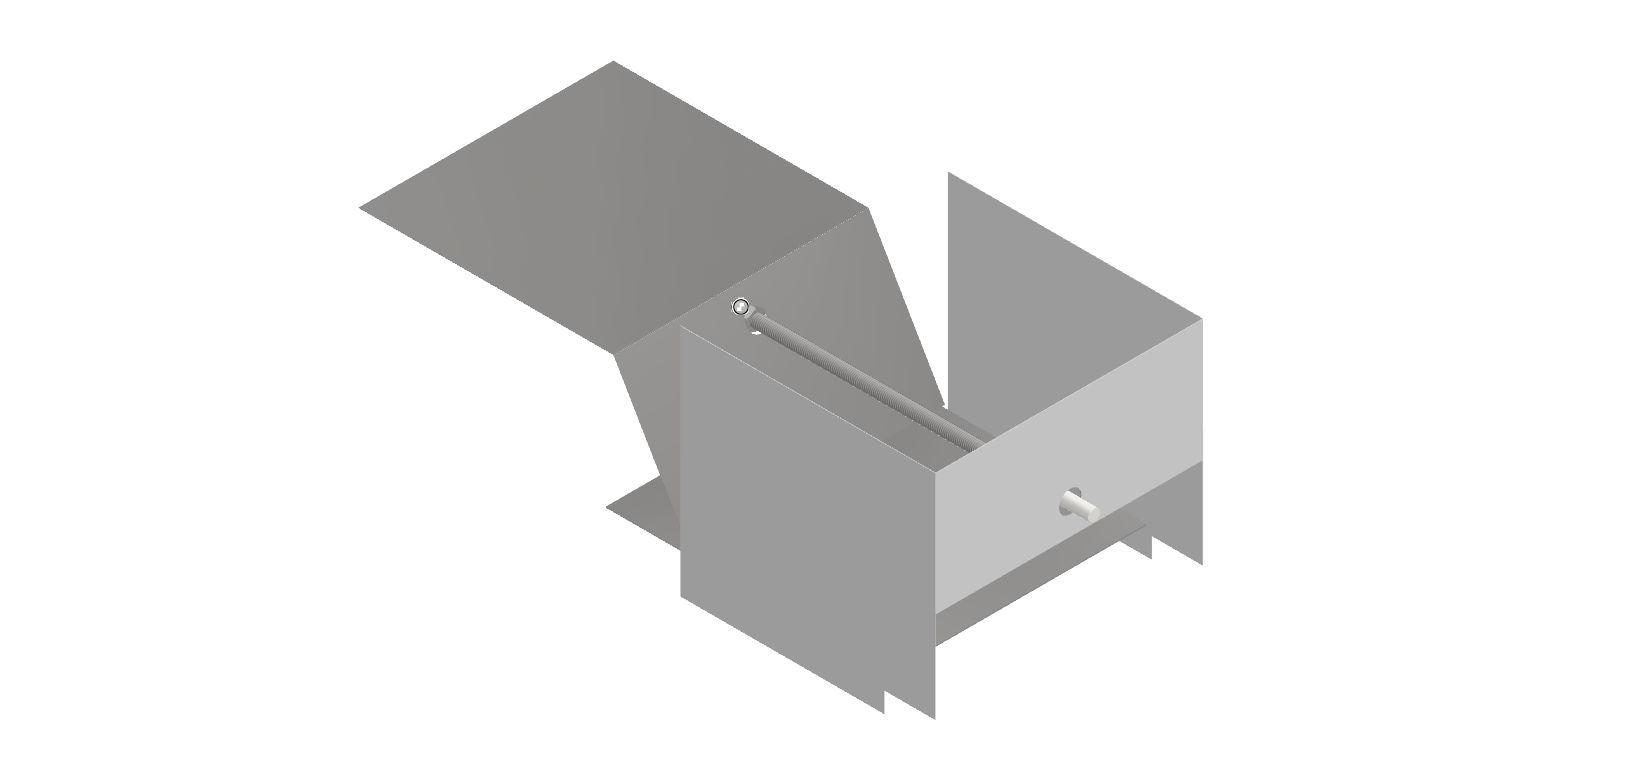
\includegraphics[width=0.45\linewidth]{imagenes/imacap/disdet/sisalim/Modulo Peso.png}}
    \subfigure[Vista lateral del módulo de pesaje.]{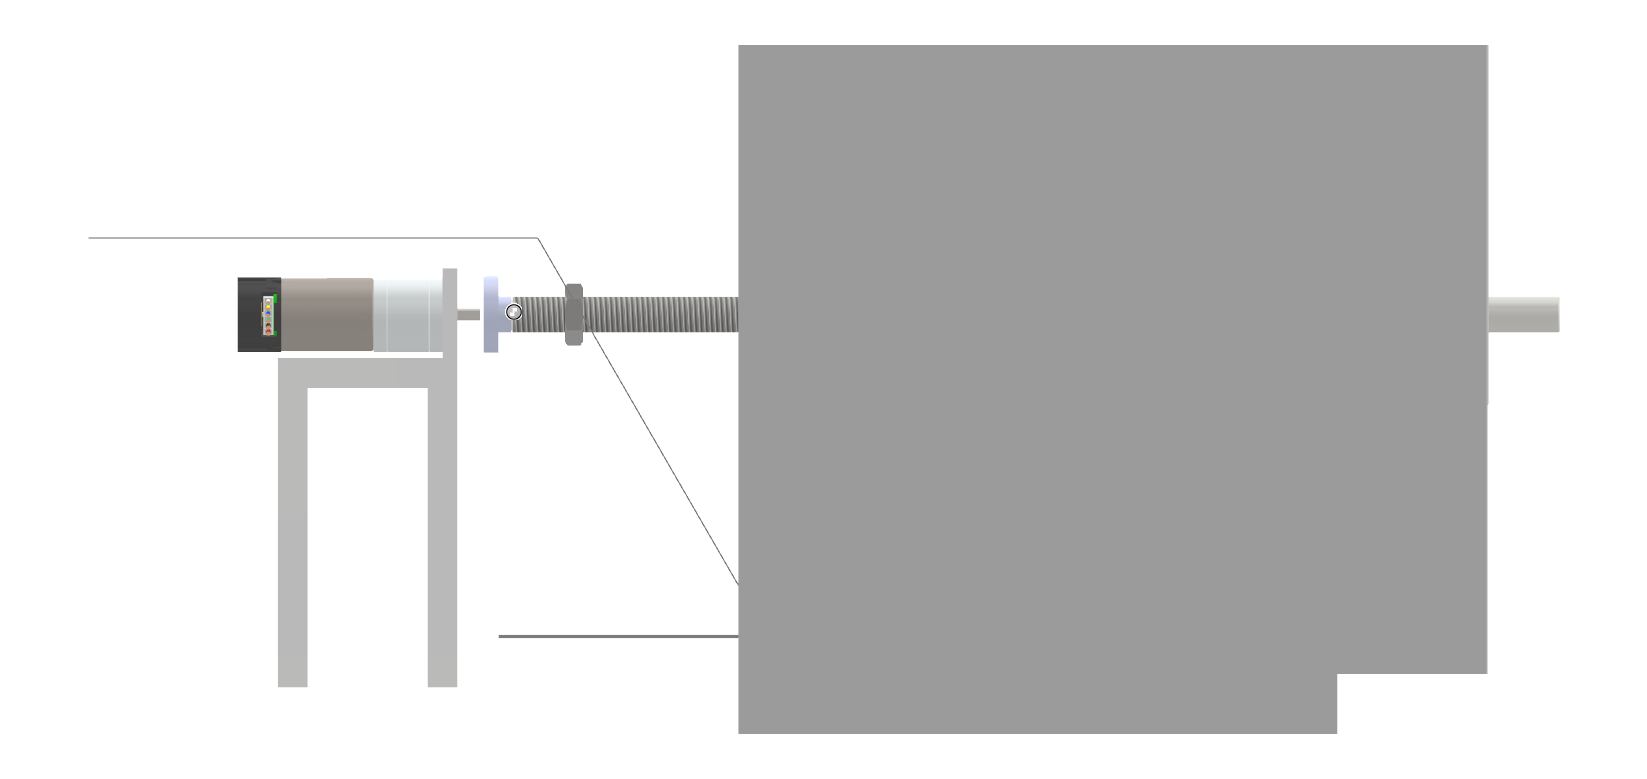
\includegraphics[width=0.5\linewidth]{imagenes/imacap/disdet/sisalim/Modulo Peso Lateral.png}}
    \caption{Módulo de pesaje.}
    \label{fig:Basc}
\end{figure}

Para mover la pared se propone el uso de un motor de C.D. con un momento de $6 \text{ Nm}$, el cual estará soportado mediante una estructura que dará la altura suficiente para empujar la pared.

%\subsubsection{Validación del módulo de pesaje}

\subsection{Distribución del alimento}

En el módulo de distribución de alimento, se propone utilizar una tolva móvil \index{tolva!móvil}, que pueda repartir una cantidad máxima de $3 \text{ kg}$ de manera uniforme a lo largo de una canaleta de la cual se alimentarán las gallinas.

Para el diseño de la tolva móvil, imagen \ref{fig:Tolva Movil}, se decide utilizar lámina de acero galvanizado, al igual que en la tolva fija; se elige utilizar una tolva con forma piramidal, con paredes rectas que permitan la sujeción de la tolva a los ejes de movimiento. 

Para definir sus dimensiones se realizó un procedimiento similar al realizado en la tolva principal. Requiriendo un volumen mínimo de $5.027\times10^{-3} \text{ m}^3 $ para contener un aproximado de $3 \text{ Kg} $ de alimento.

\begin{figure}[htbp]
    \centering
    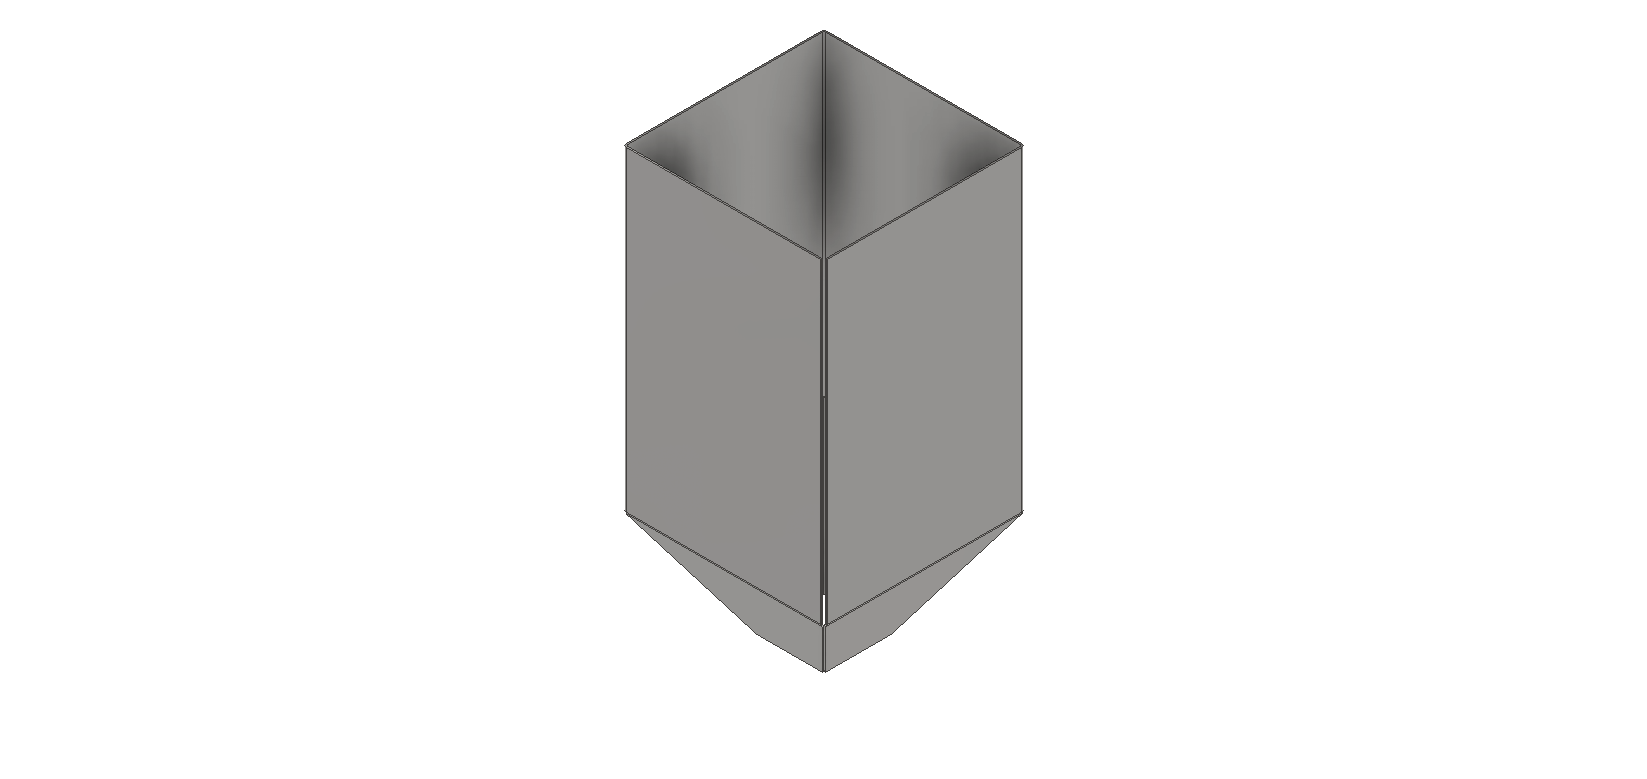
\includegraphics[width=\linewidth]{imagenes/imacap/disdet/sisalim/Tolva Movil.png}
    \caption{Modelo de la tolva móvil.}
    \label{fig:Tolva Movil}
\end{figure}

La tolva móvil se desplazará a lo largo de dos ejes, para los cuales se realizó un cálculo estático para determinar la sección transversal ideal que soportará el peso de la tolva con el alimento, para lo cual se parte de un diagrama de cuerpo libre como el que se muestra en la imagen \ref{fig:DCLTM}. 

Ubicando el centro de gravedad en el punto $(0,88)$, se determinan las direcciones de las fuerzas $A$ y $B$, con las que se busca que el sistema esté en equilibrio estático.

\begin{figure}[htbp]
    \centering
    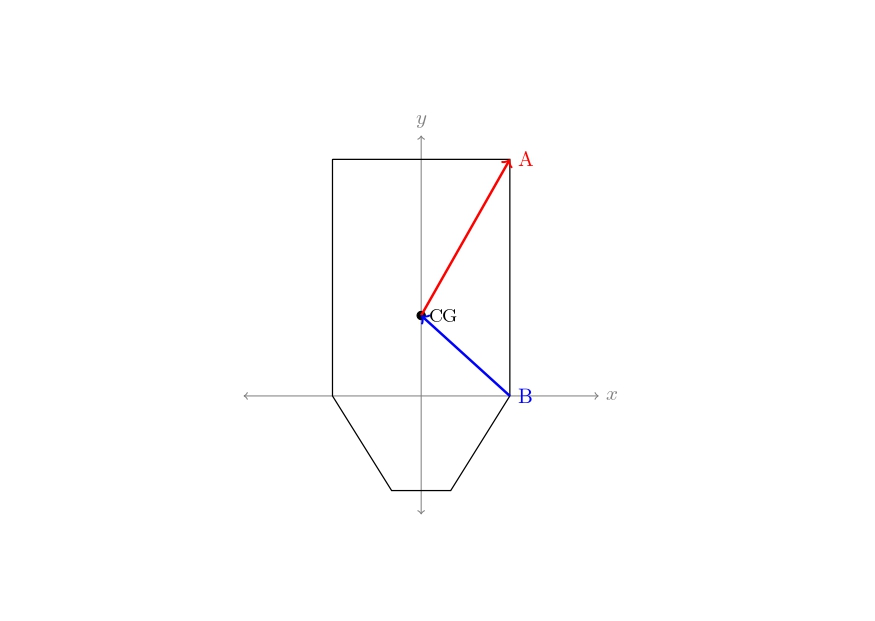
\includegraphics[width=\linewidth]{imagenes/imacap/disdet/sisalim/DCLTM.jpg}
    \caption{Diagrama cuerpo libre tolva móvil.}
    \label{fig:DCLTM}
\end{figure}

Con las condiciones de equilibrio:

\begin{align}
    \sum F_x&=A_x-B_x=0 \label{eq:Fx} \\
    \sum F_y&=A_y+B_y-W=0 \label{eq:Fy}
\end{align}

Se obtiene el valor de las fuerzas $A=42.37\text{ N}$ y $B=28.9 \text{ N} $. Dado que la fuerza en $A$ es mayor, podemos obtener la sección transversal para el eje utilizando la fuerza $A$. Proponiendo una sección transversal redonda de $25 \text{ mm}$.

La tolva se moverá por un espárrago ACME de $7/8 \text{ pulgada}$, el cual transmitirá la potencia de un motor a pasos NEMA 23, que cuenta con la fuerza suficiente para mover la carga.

El alimento será distribuido a un contenedor hecho de PVC, el cual servirá para que las gallinas puedan acercarse a comer. Dicho contenedor está soportado en dos ménsulas de PTR a una altura de $ \text{ mm}$, para que las gallinas puedan acceder fácilmente, como se muestra en la imagen \ref{fig:Canaleta}.

\begin{figure}[htbp]
    \centering
    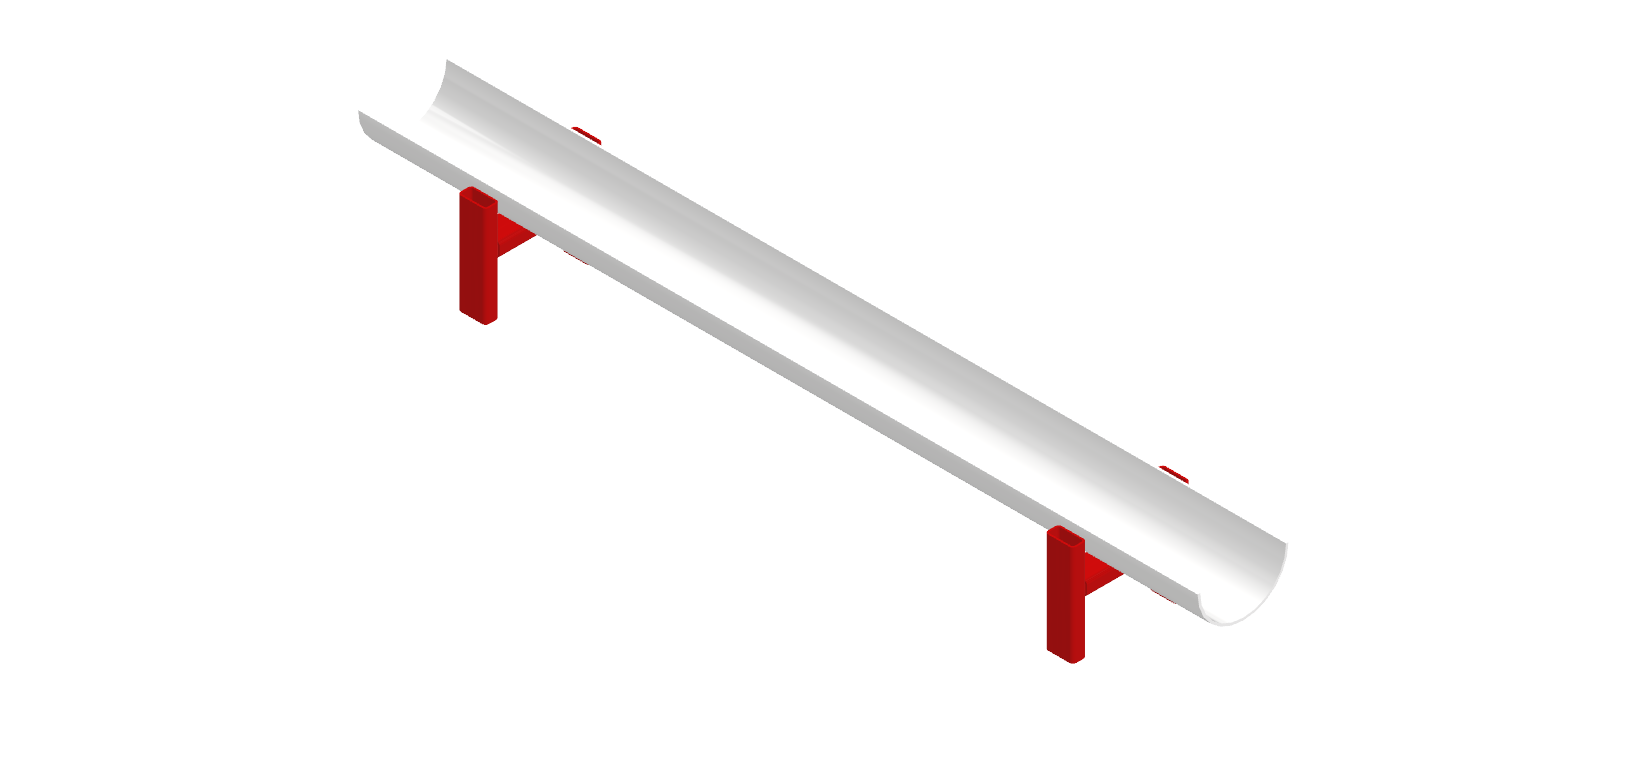
\includegraphics[width=\linewidth]{imagenes/imacap/disdet/sisalim/Canaletaens.png}
    \caption{Modelo canaleta alimentación}
    \label{fig:Canaleta}
\end{figure}


\subsubsection{Validación}

Para validar el módulo, se realiza un análisis de tensión utilizando software, con el que se obtienen los resultados de la imagen \ref{fig:TVMTM}, que indican que el diseño puede soportar el peso del alimento, al mostrar una tensión máxima de $42.38 \text{ MPa}$, estando debajo del límite elástico.

\begin{figure}[htbp]
    \centering
    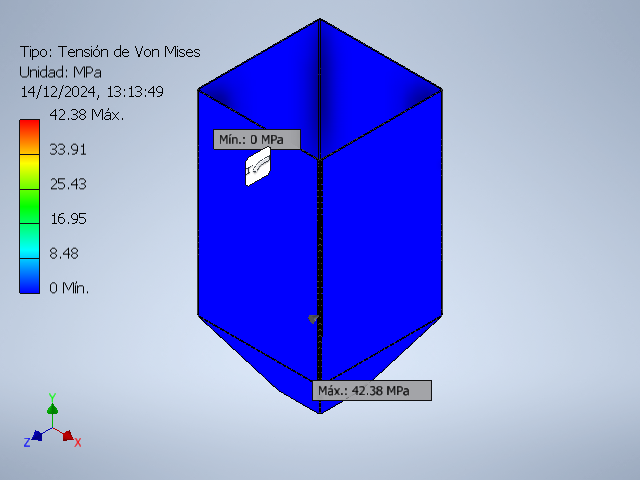
\includegraphics[width=0.8\linewidth]{imagenes/imacap/disdet/sisalim/ATVMTM.png}
    \caption{Tensión de Von Mises de la tolva móvil.}
    \label{fig:TVMTM}
\end{figure}

Los ejes se validaron utilizando la herramienta de cálculo de ejes de Autodesk Inventor. Utilizando la fuerza obtenida por las ecuaciones \eqref{eq:Fx} y \eqref{eq:Fy}. Obteniendo la gráfica de la imagen \ref{fig:FEA}, se determina que el eje tiene una flexión aceptable y soportará correctamente la tolva.

\begin{figure}[htbp]
    \centering
    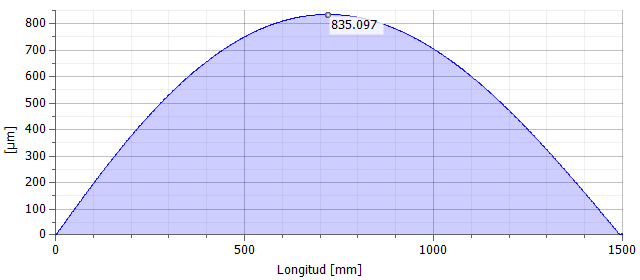
\includegraphics[width=0.8\linewidth]{imagenes/imacap/disdet/sisalim/FEA.png}
    \caption{Flexión del eje $A$.}
    \label{fig:FEA}
\end{figure}

Al igual que los ejes, la validación del tornillo se realizó utilizando la herramienta antes mencionada. Obteniendo la gráfica de la imagen \ref{fig:FT}, con la que se determina una flexión aceptable al ser menor a un milímetro.

\begin{figure}[htbp]
    \centering
    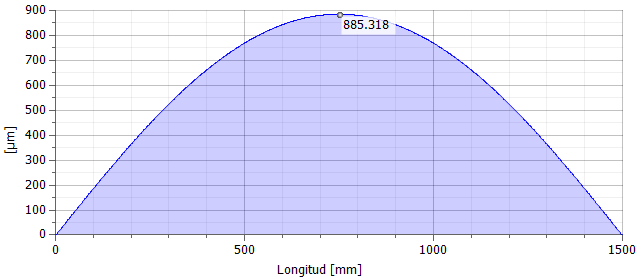
\includegraphics[width=0.8\linewidth]{imagenes/imacap/disdet/sisalim/FT.png}
    \caption{Flexión del tornillo.}
    \label{fig:FT}
\end{figure}

Al igual que en la tolva fija, se calculó un motor a pasos con un par de $0.88 \text{ Nm}$ para liberar y obstruir el alimento hacía la canaleta de alimento, y de la misma manera, el motor estará conectado con un mecanismo de piñón cremallera. El motor seleccionado es el NEMA 23, el cual tiene la fuerza suficiente para la apertura y cierre en la tolva móvil.

\subsection{Circuito sistema alimentación}

El sistema es controlado por el circuito que se muestra en la imagen \ref{fig:ECA}, utiliza como controlador una tarjeta ESP32. Dicha tarjeta permite la comunicación con distintos periféricos y cuenta con las entradas y salidas necesarias.

\begin{figure}[htbp]
    \centering
    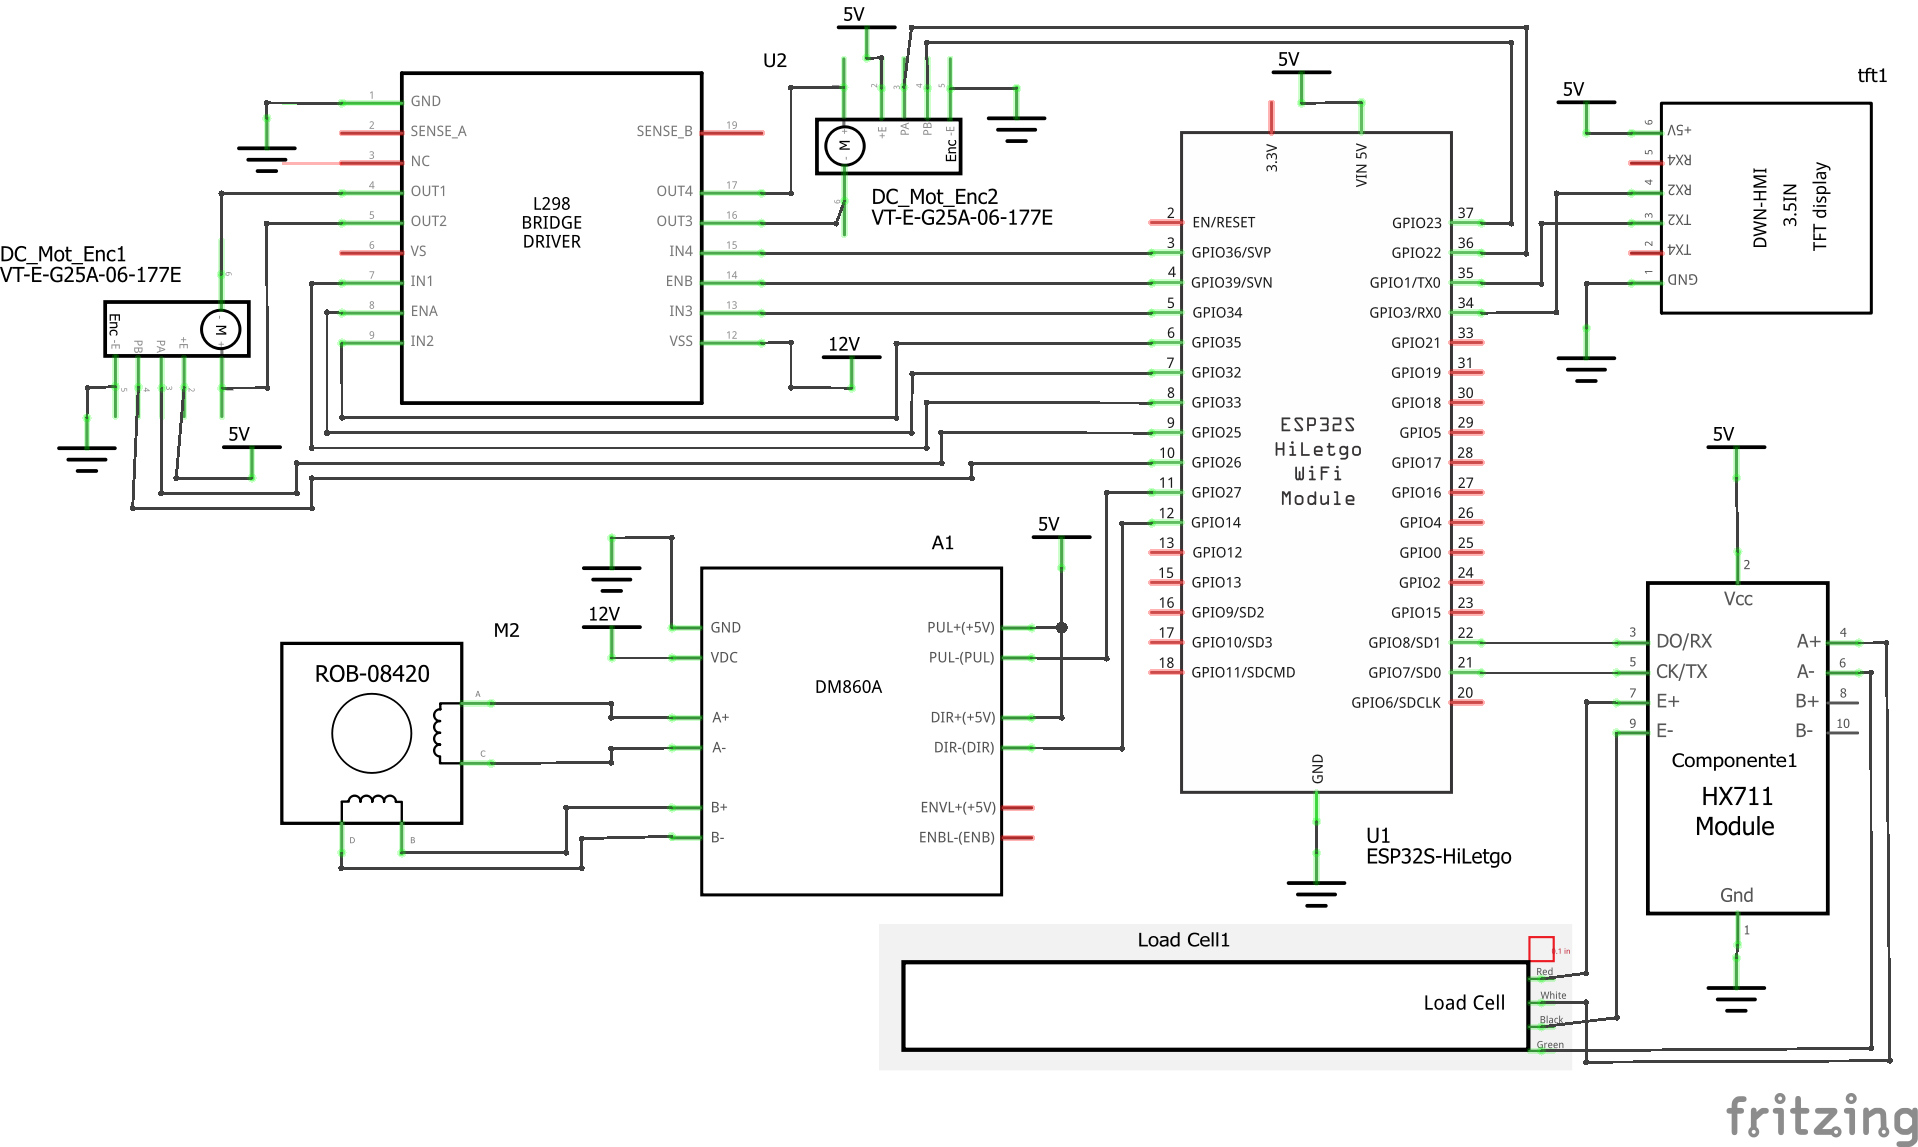
\includegraphics[width=\linewidth]{imagenes/imacap/disdet/sisalim/EsquemáticoCircuitoAlimentador.png}
    \caption{Circuito que controlará el sistema de registro de postura.}
    \label{fig:ECA}
\end{figure}

El circuito tiene como entradas el display y la celda de carga con el módulo HX711. Mientras que sus salidas son los motores junto con sus respectivos \textit{drivers}.

Se considera el uso de fuentes conmutadas para alimentar el circuito y los motores. Proporcionando así la energía necesaria. 

\subsection{Registro de postura}

El módulo de registro de postura consta de una báscula, un sensor RFID \index{RFID} y un convertidor de TTL a RS485, controlados por una tarjeta ESP32. Para el módulo se propone el uso del circuito mostrado en la imagen \ref{fig:ECR}.

\begin{figure}[htbp]
    \centering
    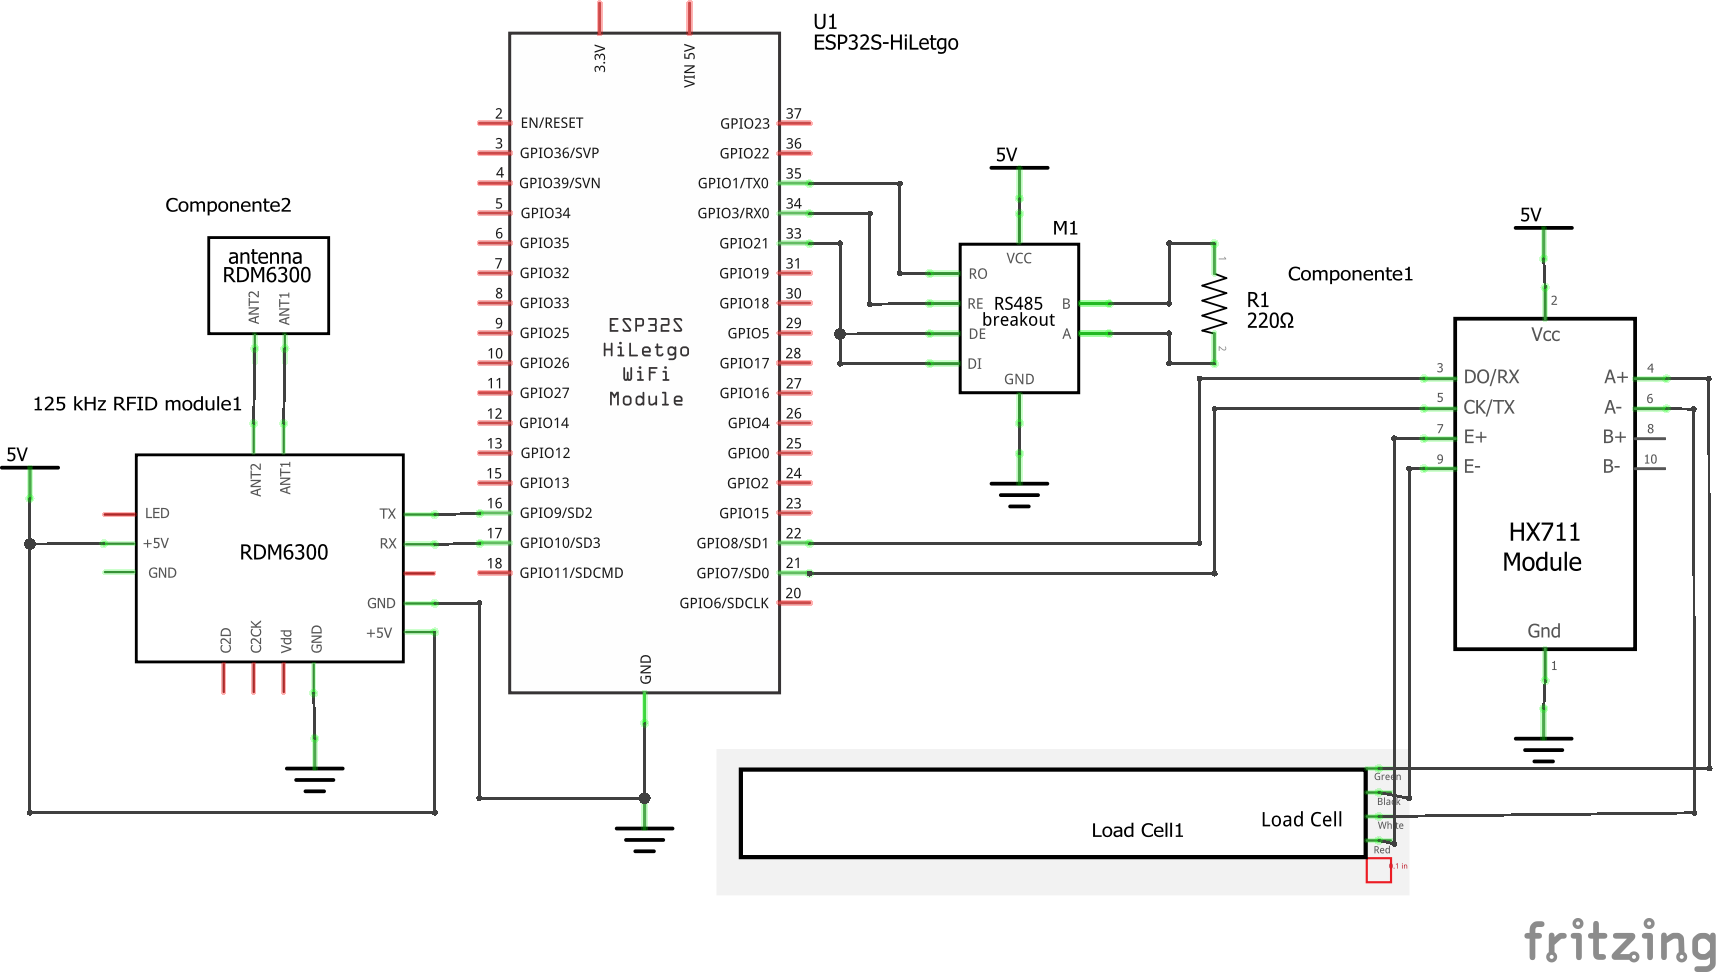
\includegraphics[width=\linewidth]{imagenes/imacap/disdet/sisreg/EsquematicoCircuitoNidal.png}
    \caption{Circuito que controlará el sistema de alimentación.}
    \label{fig:ECR}
\end{figure}

Para este sistema se considera adaptar los nidales ya existentes, colocando una lámina en el piso del nidal a modo de báscula, cubierta por paja, buscando que sea fácil de limpiar para mantener la higiene del lugar.

Debido a la cantidad de animales y su naturaleza, es necesario que cada nidal tenga un circuito individual, de tal manera que se pueda tener la información de la postura completa.

Se propone el uso de etiquetas RFID, imagen \ref{fig:RFID}, diseñadas para su uso en aves, para poder identificar a las gallinas.

\begin{figure}[htbp]
    \centering
    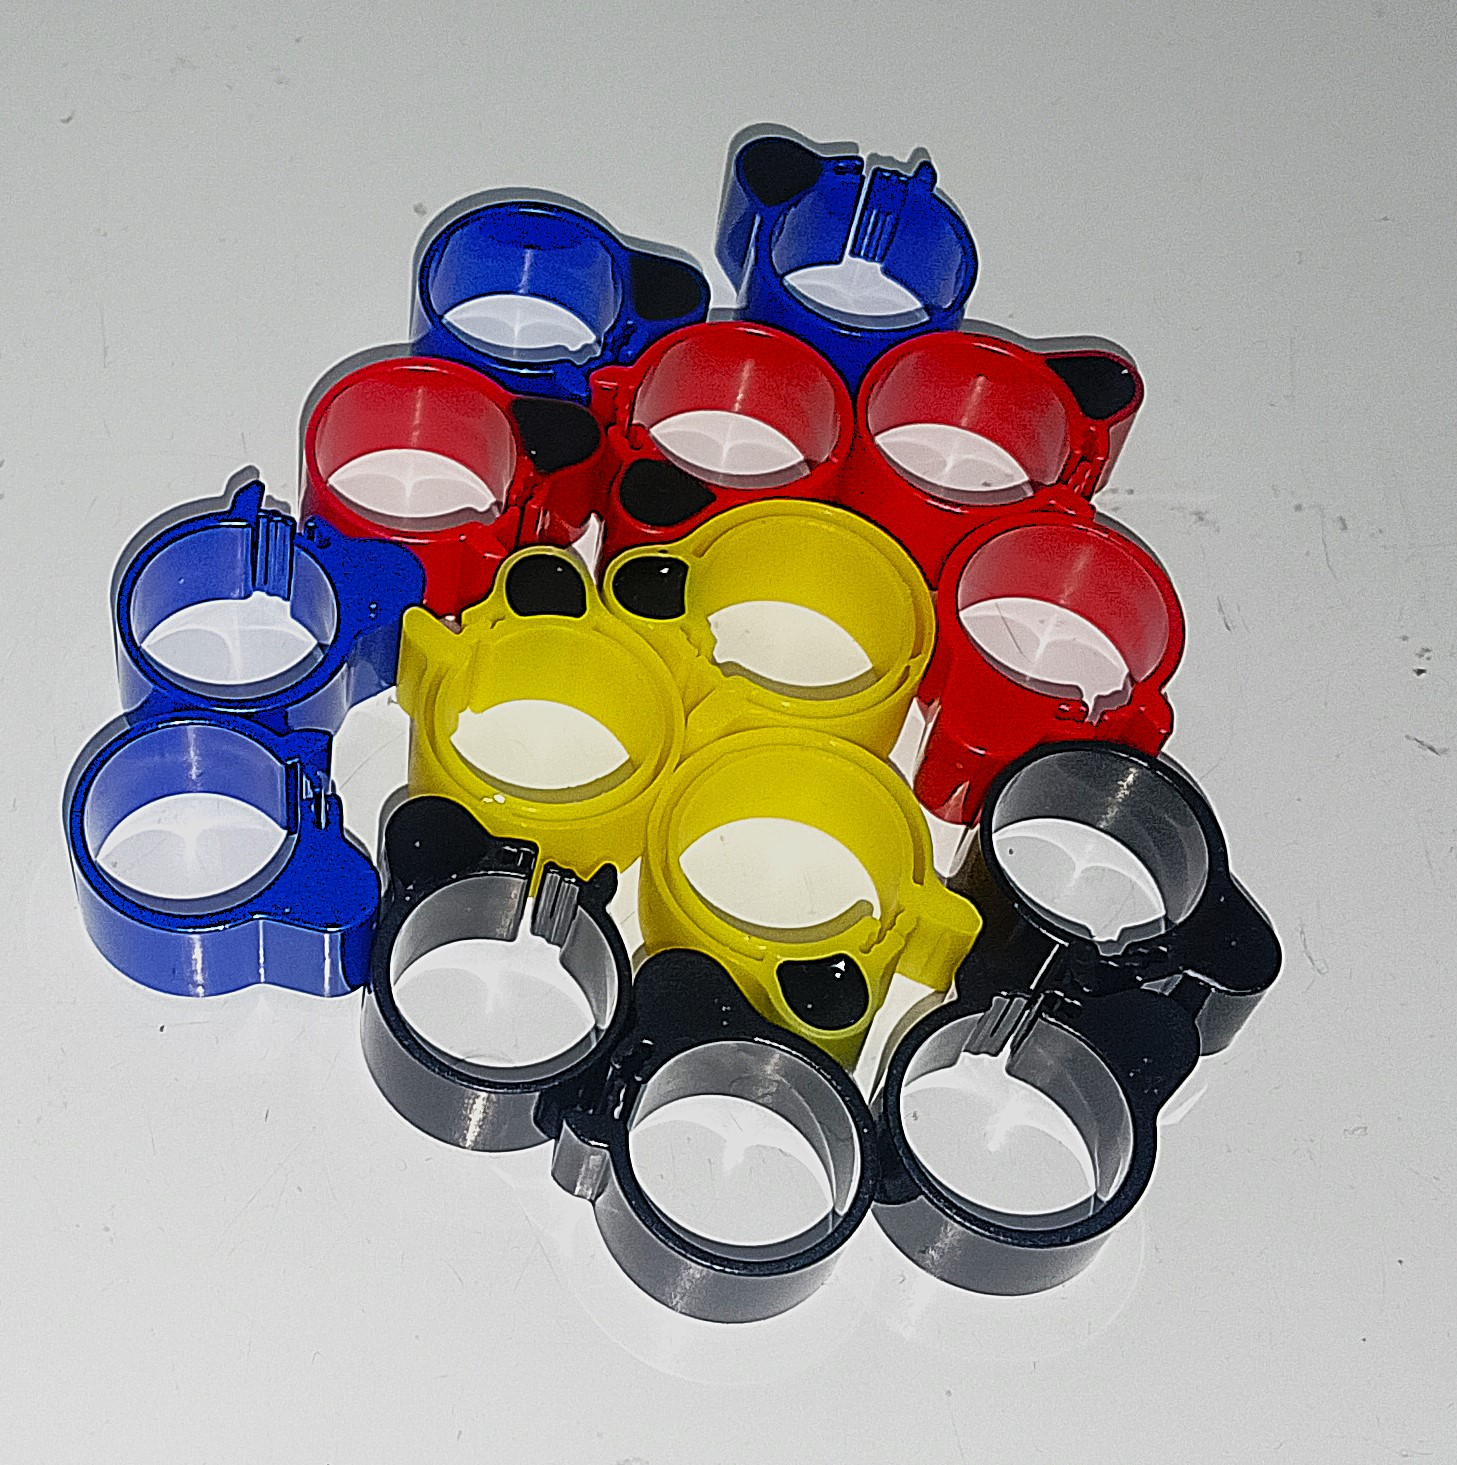
\includegraphics[width=0.3\linewidth]{imagenes/imacap/disdet/sisreg/RFID.jpg}
    \caption{Circuito que controlará el sistema de alimentación.}
    \label{fig:RFID}
\end{figure}

\subsection{Comunicación con el usuario del monitoreo de postura}

Se propone el uso del protocolo RS485 \index{RS485} en su capa física para la comunicación entre los nidales y una computadora que actuará como \textit{maestro}  del sistema, registrando y mostrando la información de postura de las gallinas. 

El protocolo permite abarcar distancias largas y utiliza una topología de bus \index{topología bus}, características ideales para la aplicación requerida.

La imagen \ref{fig:DRC} muestra un esquema de la comunicación entre dispositivos. Mientras que la tabla \ref{tab:MDI} representa los datos que serán entregados a la interfaz.

\begin{figure}[htbp]
    \centering
    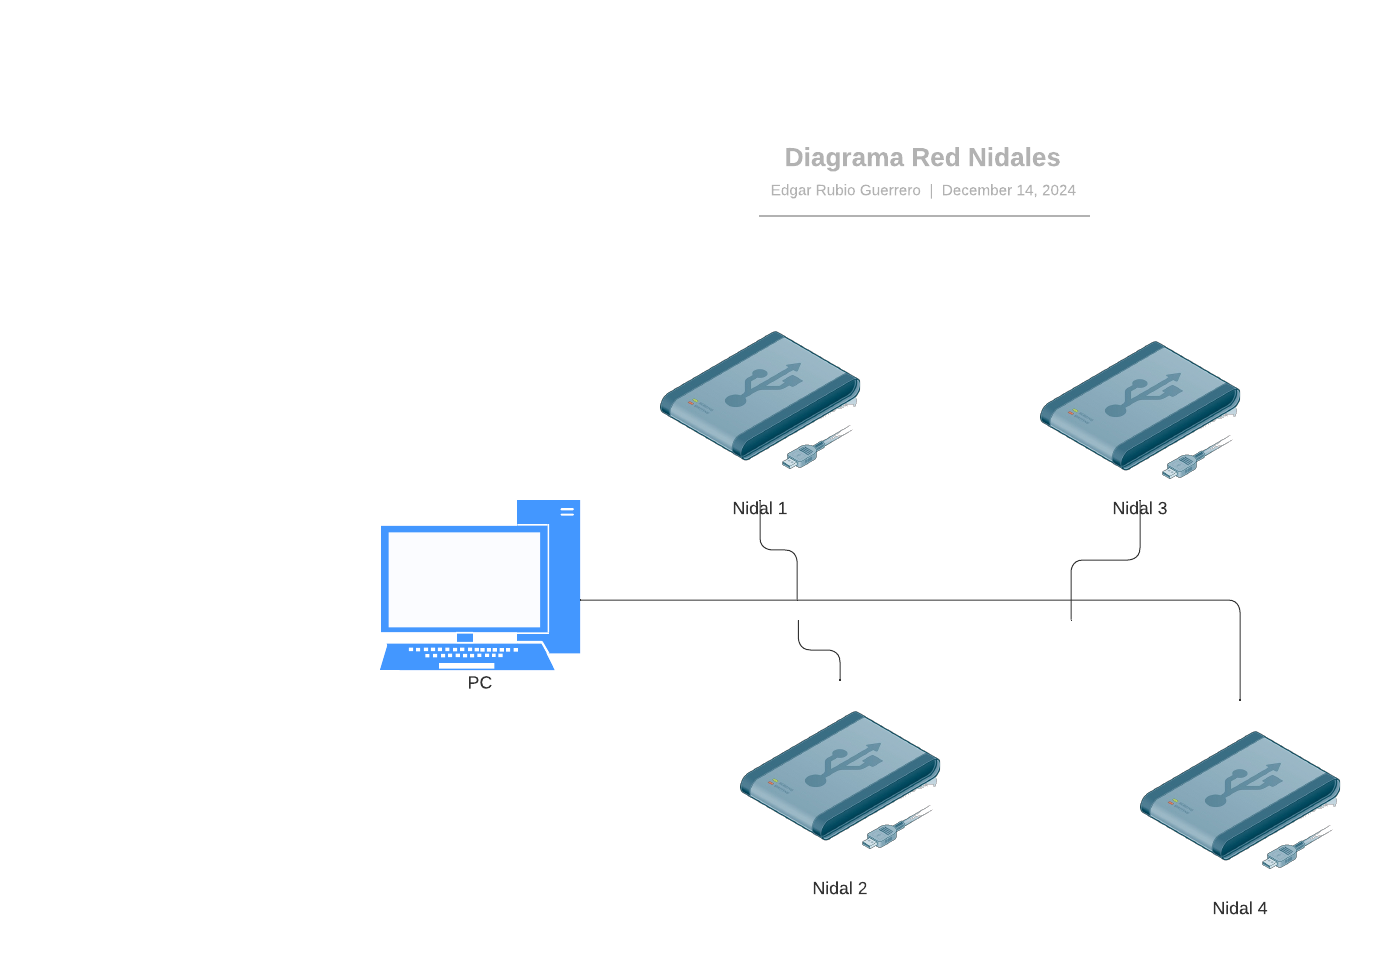
\includegraphics[width=0.6\linewidth]{imagenes/imacap/disdet/sisreg/Diagrama de red registro.png}
    \caption{Diagrama de red de los nidales con la computadora.}
    \label{fig:DRC}
\end{figure}

% Please add the following required packages to your document preamble:
% \usepackage{graphicx}
\begin{table}[htbp]
\centering
\caption{Muestreo de datos en interfaz}
\label{tab:MDI}
%\resizebox{\textwidth}{!}{%
\begin{tabular}{|l|l|l|l|}
\hline
\multicolumn{1}{|c|}{\textbf{Fecha}} &
  \multicolumn{1}{c|}{\textbf{ID}} &
  \multicolumn{1}{c|}{\textbf{Postura}} &
  \multicolumn{1}{c|}{\textbf{\begin{tabular}[c]{@{}c@{}}Ultima\\ Postura\end{tabular}}} \\ \hline
DD-MM & GXX & 1/0 & DD-MM \\ \hline
12/04 & G01 & 1   & 12/04 \\ \hline
12/04 & G20 & 0   & 11/04 \\ \hline
12/04 & G17 & 0   & 5/04  \\ \hline
      &     &     &       \\ \hline
\end{tabular}%
%}
\end{table}

\subsection{Integración sistema alimentación}

Las imágenes \ref{fig:ISA0}, \ref{fig:ISA1} y \ref{fig:ISA2} , muestran diferentes vistas de la integración del sistema de alimentación y el ensamble de los módulos y elementos que lo componen. Los planos y esquemáticos se pueden ver en los apéndices \ref{apendice1} y \ref{apendice2}

\begin{figure}[htbp]
    \centering
    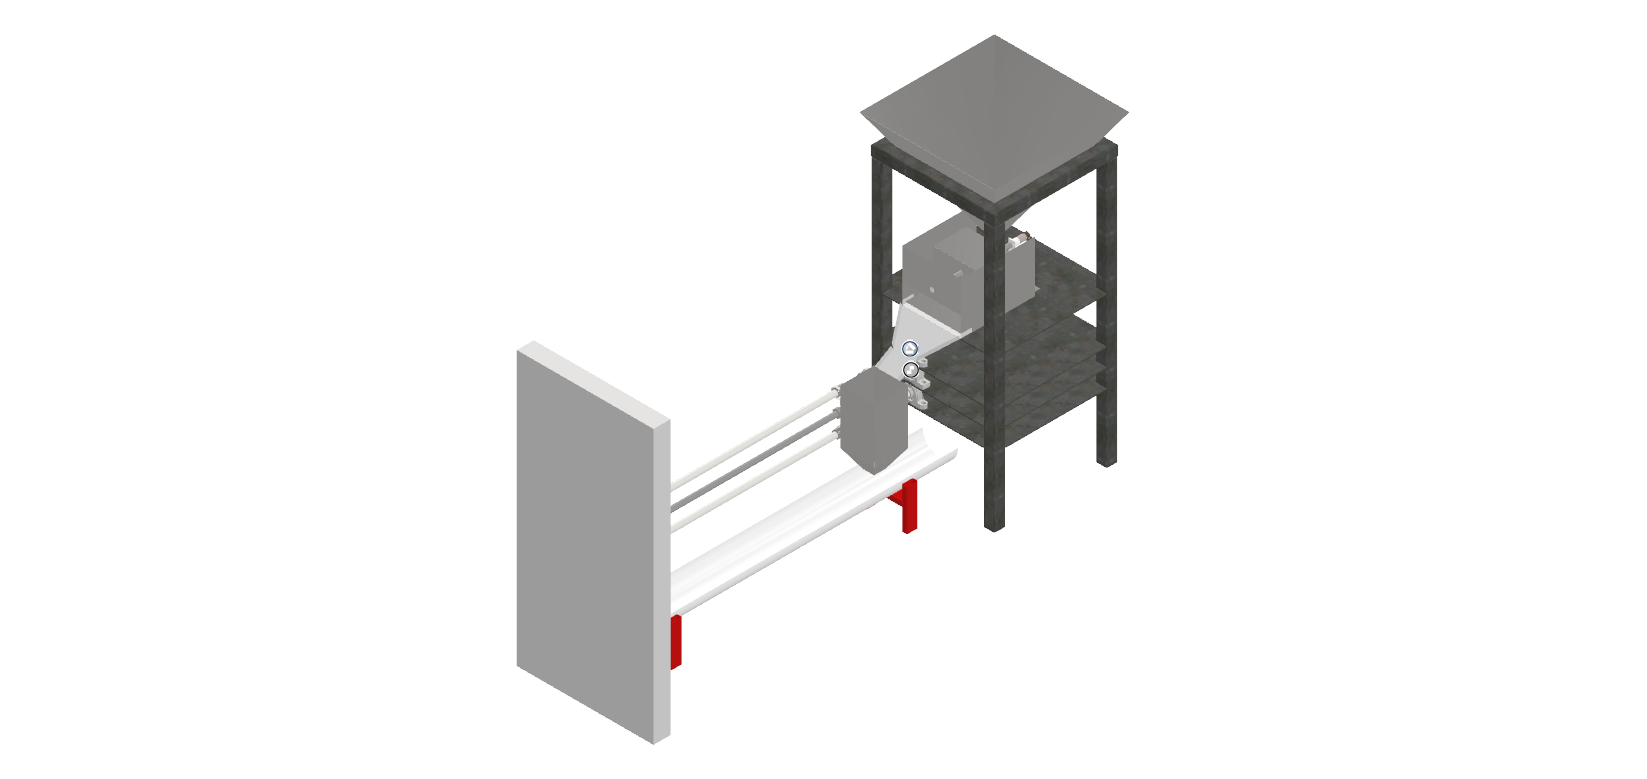
\includegraphics[width=\linewidth]{imagenes/imacap/disdet/integ/Ensamblaje Final1.png}
    \caption{Diagrama de red de los nidales con la computadora.}
    \label{fig:ISA0}
\end{figure}

\begin{figure}[htbp]
    \centering
    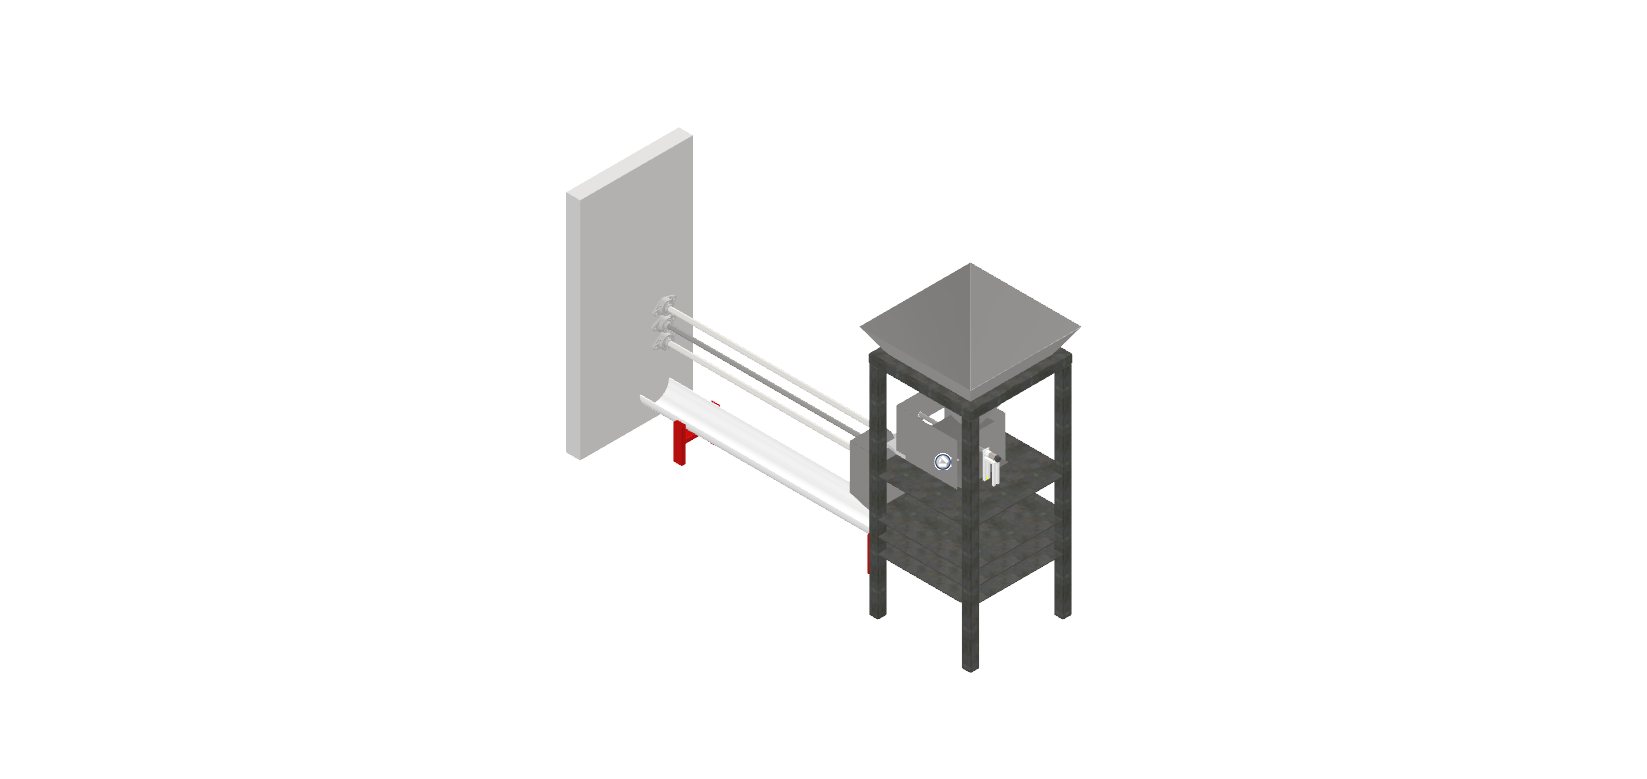
\includegraphics[width=\linewidth]{imagenes/imacap/disdet/integ/Ensamblaje Final2.png}
    \caption{Diagrama de red de los nidales con la computadora.}
    \label{fig:ISA1}
\end{figure}

\begin{figure}[htbp]
    \centering
    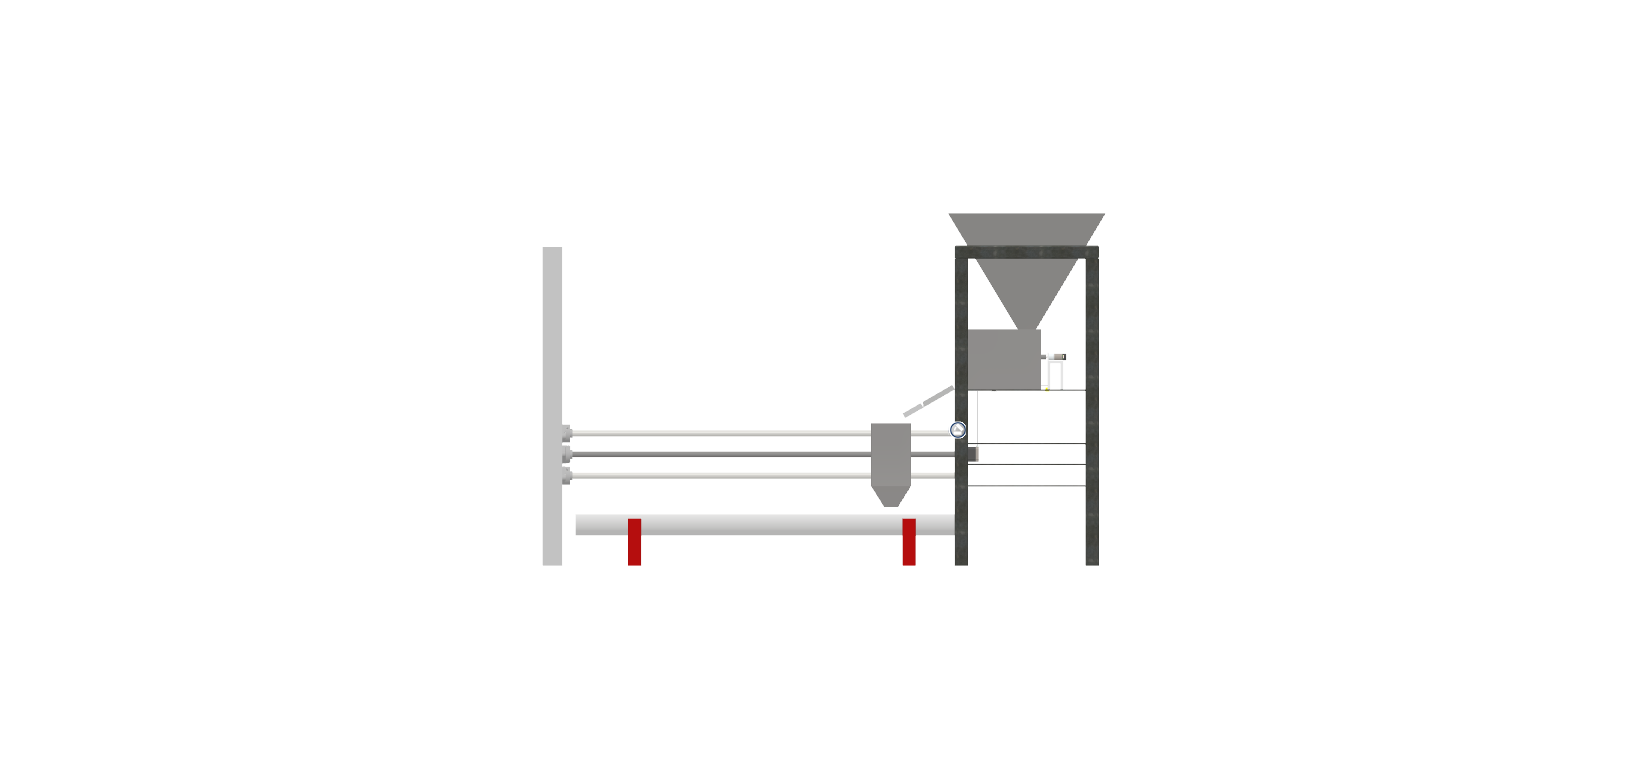
\includegraphics[width=\linewidth]{imagenes/imacap/disdet/integ/Ensamblaje Final3.png}
    \caption{Diagrama de red de los nidales con la computadora.}
    \label{fig:ISA2}
\end{figure}

%\subsection{Validación sistema mecatrónico}



%%%%%%fin del archivo
\endinput 